\documentclass[
	classe=$1^{ere}STI2D$,
	landscape,
	twocolumn,
]{évaluation}

\setlength{\columnsep}{1cm}
\renewcommand{\arraystretch}{1.4}

\date{5 mai 2023}

\begin{document}

\title{Interrogation : Probabilités (Sujet A)}
\maketitle

\begin{center}
	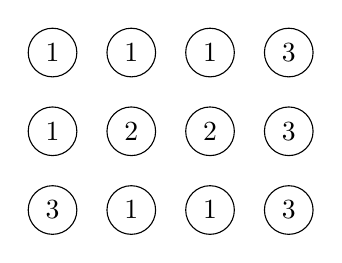
\begin{tikzpicture}
		\foreach \x/\y/\a in {0/0/3,1/0/1,2/0/1,3/0/3,0/1/1,1/1/2,2/1/2,3/1/3,0/2/1,1/2/1,2/2/1,3/2/3} {
				\node[shape=circle,draw=black] at (\x,\y) {$\a$};
			}
	\end{tikzpicture}
\end{center}
On tire aléatoirement un jeton numéroté parmi l'ensemble ci-dessus, puis on le repose, et on en tire un deuxième.
\begin{enumerate}
	\item Quelles sont les issues possibles d'un seul tirage ?
	\item Représenter les deux tirages avec un arbre de probabilités.
	\item Quelle est la probabilité de tirer un $1$, puis un $3$ ?
	\item Quelle est la probabilité de tirer exactement un $2$ (ni plus, ni moins) ?
	\item On fait maintenant le paris suivant :

	      Si on tire deux $3$ de suite, on gagne $10$€. Sinon, on perd $5$€.

	      On note $X$ la variable aléatoire associée au gain. Quelles sont les valeurs possibles de $X$ ?
	\item Donner la valeur de $P(X = 10)$.
\end{enumerate}

%=============================================
%================= SUJET B ===================
%=============================================

\newpage

\title{Interrogation : Probabilités (Sujet B)}
\maketitle

\begin{center}
	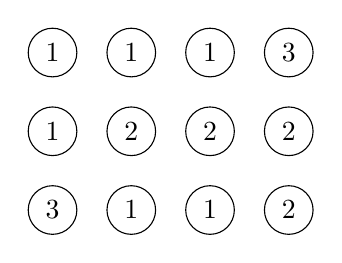
\begin{tikzpicture}
		\foreach \x/\y/\a in {0/0/3,1/0/1,2/0/1,3/0/2,0/1/1,1/1/2,2/1/2,3/1/2,0/2/1,1/2/1,2/2/1,3/2/3} {
				\node[shape=circle,draw=black] at (\x,\y) {$\a$};
			}
	\end{tikzpicture}
\end{center}
On tire aléatoirement un jeton numéroté parmi l'ensemble ci-dessus, puis on le repose, et on en tire un deuxième.
\begin{enumerate}
	\item Quelles sont les issues possibles d'un seul tirage ?
	\item Représenter les deux tirages avec un arbre de probabilités.
	\item Quelle est la probabilité de tirer un $1$, puis un $3$ ?
	\item Quelle est la probabilité de tirer exactement un $2$ (ni plus, ni moins) ?
	\item On fait maintenant le paris suivant :

	      Si on tire deux $3$ de suite, on gagne $20$€. Sinon, on perd $5$€.

	      On note $X$ la variable aléatoire associée au gain. Quelles sont les valeurs possibles de $X$ ?
	\item Donner la valeur de $P(X = 20)$.
\end{enumerate}

\end{document}